\documentclass[10pt,a4paper]{article}
\usepackage{verbatim}
\usepackage{subcaption}
\usepackage{karnaugh-map}
\usepackage[utf8]{inputenc}
\usepackage[italian]{babel}
\usepackage{amsmath}
\usepackage{amsfonts}
\usepackage{amssymb}
\usepackage{graphicx}
\usepackage[left=2cm,right=2cm,top=2cm,bottom=2cm]{geometry}
\newcommand{\rem}[1]{[\emph{#1}]}
\newcommand{\exn}{\phantom{xxx}}
\renewcommand{\thesubsection}{\thesection.\alph{subsection}}  %% use 1.a numbering

\author{Gruppo EB.24 \\Giovanni Sucameli, Davide Incalza, Francesco Sacco}
\title{Effetto fotoelettrico - Misura del rapporto $\frac{h}{e}$}
\begin{document}
\date{25 Marzo 2019}
\maketitle
\section*{Scopo dell'esperienza e cenni teorici}
Obiettivo di questa esperienza è la verifica dell'effetto fotoelettrico e dell'ipotesi di Einstein (1905) e successivamente verificata da Einstein, secondo cui un'onda elettromagnetica è costituita da quanti di luce, detti fotoni, ciascuno dei quali porta un energia 

\begin{equation}
 E_{\gamma} = h\nu
\label{energia}
\end{equation}

dove h è la costante di Planck e $ \nu $ la frequenza dell'onda. Affinchè un elettrone venga estratto dal metallo è necessario che assorba un fotone di energia superiore al lavoro $ W_{0}$ di estrazione dal metallo ( $ W_{0} $)  varia da metallo a metallo). Dunque l'energia cinetica del fotoelettrone è data da
\begin{equation}
    E_{e} = hv - W_{0}
\label{foto}
\end{equation}
Da quest'ultima equazione ricaveremo poi anche una stima del rapporto $ \frac{h}{e} $
Notiamo infine che, secondo l'ipotesi di Einstein, l'intensità della corrente formata dai fotoelettroni è proporzionale al numero di fotoni (con energia tale da estrarre l'elettrone dal metallo) incidenti sul metallo nell'unità di tempo.

\section*{Materiale occorrente}

\begin{itemize}
\item una lampada a led
\item una fotocella Leybold 55877 
\item filtri interferenziali (Newport)
\item scatola metallica
\item generatore di tensione continua
\item un multimetro digitale
\item un picoamperometro digitale
\end{itemize}

\section*{Esperimento di Millikan}
Robert Millikan (che già nel 1909 aveva misurato la carica elementare) tra il 1914 ed il 1916 effettuò misure per verificare l'ipotesi di Einstein. L'idea di Millikan è quella di far incidere della luce di frequenza $\nu$ (che può essere variata) su un bulbo di vetro su cui era stato depositato a vuoto un catodo alcalino. La corrente dovuta ai fotoelettroni poteva essere misurata mediante un mllliamperometro chiuso su un generatore di tensione continua in grado di generare una d.d.p. continua tra il catodo e l'anodo; la polarità è tale da generare nel bulbo un campo elettrico opposto al flusso dei fotoelettroni verso l'anodo, in modo di diminuire la corrente nel circuito. Regolando la tensione V fino ad un valore $V_{0}$ tale da annulare la corrente, si ottiene una stima dell'energia cinetica massima dei fotolettroni da mettere in relazione alla frequenza della luce (per verificare la linearità della relazione energia-frequenza (equazione \ref{foto}), e ottenere una stima del rapporto $\frac{h}{e}$ ). 
%\newline \newline
\section*{Apparato sperimentale}
Per la verifica dell'equazione (\ref{foto}) abbiamo utilizzato un metodo simile a quello usato da Millikan. L'apparato sperimentale è composto da :

\begin{itemize}
\item una fotocella Leybold 55877
\item una lampada a led usata come sorgente di luce con uno spettro quasi continuo
\item un set di filtri interferenziali con cui variare la frequenza dell'onda incidente sul catodo (i valori delle lunghezze d'onda centrali e delle bande passanti sono in Tab.\ref{tab:filtri} )
\item un generatore di tensione continua (da banco) per variare la tensione di bias tra catodo e anodo
\item un voltmetro digitale per misurare la tensione di bias all'uscita del generatore
\item un picoamperometro per misurare la corrente dei fotoelettroni
\end{itemize}

\begin{table}[h]
\caption{\small Lunghezza d'onda centrali, rispettive frequenze con incertezze di banda associate e colore della luce in uscita per i filtri utilizzati. }
\label{tab:filtri}
\begin{center}
\begin{tabular}{|c|c|c|c|c|}
\hline
colore & $\lambda$ (nm) & FWHM (nm) & $\nu (10^{14} $ Hz ) & d$\nu$   \\
\hline 
azzurro & 450.9 & 9.6 & & \\
\hline
verde-azzurro & 499.05 & 11.10 & &\\
\hline
verde & 546.03  & 11.68 & &\\
\hline
giallo & 577  &  10 & & \\
\hline
\end{tabular}
\end{center}
\end{table}

\begin{figure}[h]
\begin{center}
\includegraphics[width=0.5\linewidth]{circuito_equivalente.png}
\caption{\small Schema elettrico equivalente per la misura dell'energia cinetica dei fotoni. }
\label{fig:cireq}
\end{center}
\end{figure}

\begin{figure}[h]
\begin{center}
\includegraphics[width=0.5\linewidth]{schema_banco.png}
\caption{\small Schema del banco ottico. }
\label{fig:schemabanco}
\end{center}
\end{figure}

\newpage
\section*{Analisi Dati}
\begin{minipage}{.6\linewidth}
		\centering
		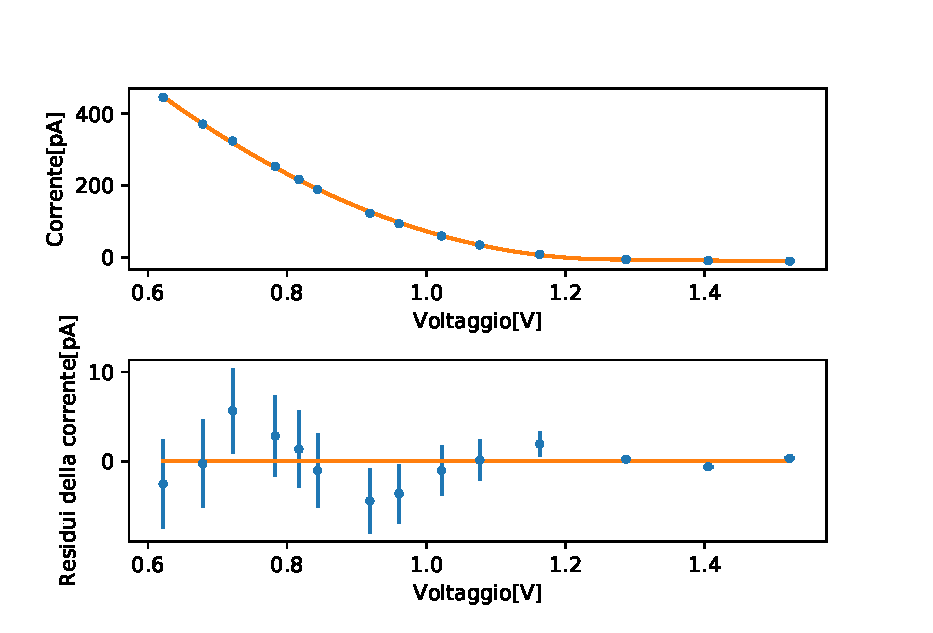
\includegraphics[width=\linewidth]{450nm.eps}
		\captionof{figure}{Circuito usato nel punto 1}
		\label{fig:circuito-1}
	\end{minipage}
	\begin{minipage}{.4\linewidth}
		\begin{tabular}{cc}
\hline
	Parametri di Fit & Valori di Fit\\ 
\hline
	$V_0$ & $1.26\pm0.006$ \\
	$a$ & $(-1.08\pm0.03)\times 10^{-9}$ \\
	$b$ & $(2.0\pm0.2)\times 10^{-11}$ \\
	$I_0$ & $(-2.0\pm0.2)\times 10^{-11}$ \\
	$\chi^2$ & $23.88$ \\
\hline
\end{tabular}

		\label{tab:124}
\end{minipage}\newline\newline
\begin{minipage}{.6\linewidth}
		\centering
		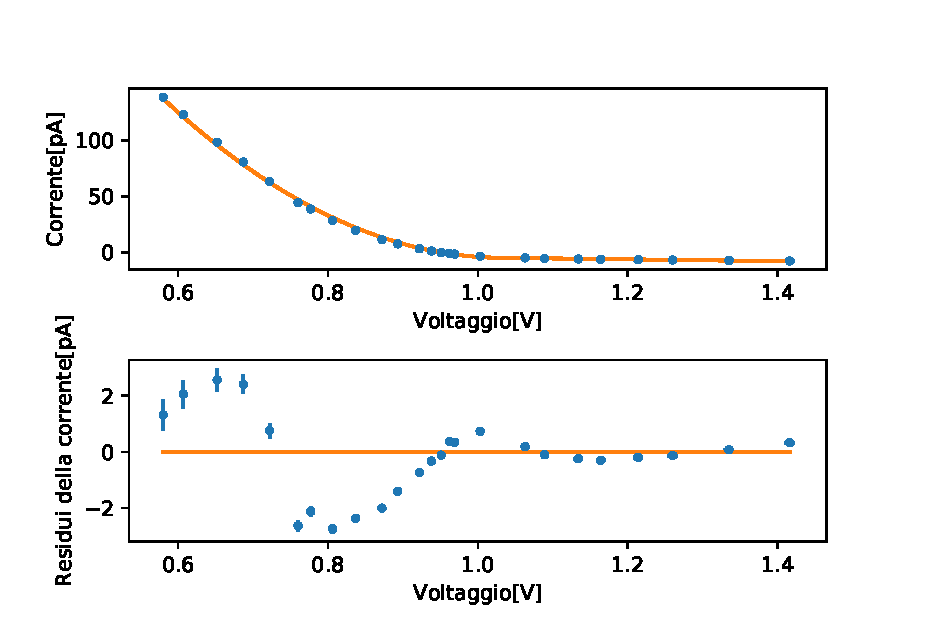
\includegraphics[width=\linewidth]{499nm.eps}
		\captionof{figure}{Circuito usato nel punto 1}
		\label{fig:circuito-1}
	\end{minipage}
	\begin{minipage}{.4\linewidth}
		\begin{tabular}{cc}
\hline
	Parametri di Fit & Valori di Fit\\ 
\hline
	$V_0$ & $1.029$ $\pm$ $0.002$ \\
	$a$ & $(-6.9$ $\pm$ $0.1)\times 10^{-10}$ \\
	$b$ & $(8.0$ $\pm$ $0.4)\times 10^{-12}$ \\
	$I_0$ & $(-3.5$ $\pm$ $0.4)\times 10^{-12}$ \\
	$\chi^2$ & $6.43\times 10^{1}$ \\
\hline
\end{tabular}

		\label{tab:124}
\end{minipage}\newline\newline
\begin{minipage}{.6\linewidth}
		\centering
		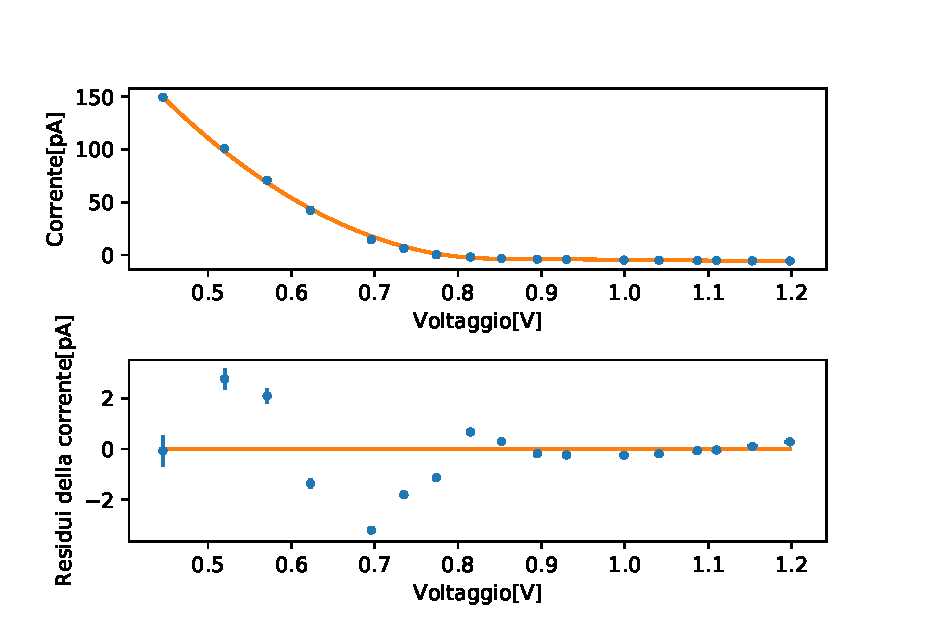
\includegraphics[width=\linewidth]{545nm.eps}
		\captionof{figure}{Circuito usato nel punto 1}
		\label{fig:circuito-1}
	\end{minipage}
	\begin{minipage}{.4\linewidth}
		\begin{tabular}{cc}
\hline
	Parametri di Fit & Valori di Fit\\ 
\hline
	$V_0$ & $0.841$ $\pm$ $0.002$ \\
	$a$ & $(-9.7$ $\pm$ $0.2)\times 10^{-10}$ \\
	$b$ & $(7.1$ $\pm$ $0.3)\times 10^{-12}$ \\
	$I_0$ & $(-2.4$ $\pm$ $0.3)\times 10^{-12}$ \\
	$\chi^2$ & $61.8$ \\
\hline
\end{tabular}

		\label{tab:124}
\end{minipage}\newline\newline
\newline
\begin{minipage}{.6\linewidth}
		\centering
		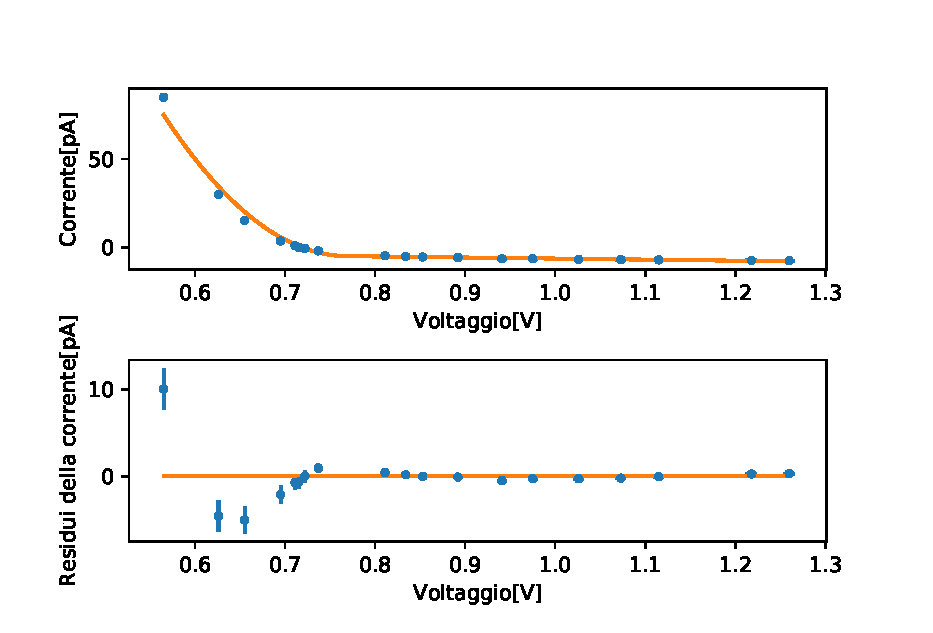
\includegraphics[width=\linewidth]{577nm.eps}
		\captionof{figure}{Circuito usato nel punto 1}
		\label{fig:circuito-1}
	\end{minipage}
	\begin{minipage}{.4\linewidth}
		\begin{tabular}{cc}
\hline
	Parametri di Fit & Valori di Fit\\ 
\hline
	$V_0$ & $0.759\pm0.01$ \\
	$a$ & $(-2.2\pm0.4)\times 10^{-9}$ \\
	$b$ & $(7.0\pm0.7)\times 10^{-12}$ \\
	$I_0$ & $(-4.0\pm7.0)\times 10^{-13}$ \\
	$\chi^2$ & $3.37\times 10^{2}$ \\
\hline
\end{tabular}

		\label{tab:124}
\end{minipage}\newline\newline
\newline
\section*{Appendice: Dati}
\noindent
Di seguito: i dati sperimentali V/I per ciascuna frequenza incidente.\\
\paragraph{Luce a 450nm:}
\begin{tabular}{cccc}
\hline
	$V[mV]$ & $\sigma V[mV]$ & $I[pA]$ & $\sigma I[pA]$\\ 
\hline
	$622$ & $3$ & $-445$ & $2$ \\
	$679$ & $3$ & $-371$ & $1$ \\
	$722$ & $3$ & $-324$ & $1$ \\
	$783$ & $4$ & $-253$ & $1$ \\
	$817$ & $4$ & $-217$ & $1$ \\
	$844$ & $4$ & $-189$ & $1$ \\
	$919$ & $4$ & $-122.7$ & $0.5$ \\
	$961$ & $4$ & $-93.6$ & $0.4$ \\
	$1022$ & $5$ & $-59.5$ & $0.3$ \\
	$1077$ & $5$ & $-34.5$ & $0.2$ \\
	$1163$ & $5$ & $-8.5$ & $0.1$ \\
	$1287$ & $6$ & $5.9$ & $0.1$ \\
	$1405$ & $7$ & $9.1$ & $0.1$ \\
	$1522$ & $7$ & $10.5$ & $0.1$ \\
\hline
\end{tabular}


\paragraph{Luce a 499nm:}
\begin{tabular}{cccc}
\hline
	$V[mV]$ & $dV[mV]$ & $I[pA]$ & $dI[pA]$\\ 
\hline
	$580$ & $3$ & $-138.4$ & $0.6$ \\
	$607$ & $3$ & $-122.8$ & $0.5$ \\
	$652$ & $3$ & $-98.3$ & $0.4$ \\
	$687$ & $3$ & $-80.6$ & $0.3$ \\
	$722$ & $3$ & $-63.1$ & $0.3$ \\
	$760$ & $3$ & $-44.4$ & $0.2$ \\
	$777$ & $4$ & $-38.7$ & $0.2$ \\
	$806$ & $4$ & $-28.4$ & $0.2$ \\
	$837$ & $4$ & $-19.7$ & $0.1$ \\
	$872$ & $4$ & $-11.4$ & $0.1$ \\
	$893$ & $4$ & $-7.6$ & $0.1$ \\
	$922$ & $4$ & $-3.2$ & $0.1$ \\
	$938$ & $4$ & $-1.3$ & $0.1$ \\
	$951$ & $4$ & $0.1$ & $0.1$ \\
	$962$ & $4$ & $0.8$ & $0.1$ \\
	$969$ & $4$ & $1.5$ & $0.1$ \\
	$1003$ & $5$ & $3.4$ & $0.1$ \\
	$1063$ & $5$ & $4.9$ & $0.1$ \\
	$1089$ & $5$ & $5.4$ & $0.1$ \\
	$1134$ & $5$ & $5.9$ & $0.1$ \\
	$1164$ & $5$ & $6.2$ & $0.1$ \\
	$1214$ & $6$ & $6.5$ & $0.1$ \\
	$1260$ & $6$ & $6.8$ & $0.1$ \\
	$1335$ & $6$ & $7.2$ & $0.1$ \\
	$1416$ & $7$ & $7.6$ & $0.1$ \\
\hline
\end{tabular}


\paragraph{Luce a 545nm:}
\begin{tabular}{cccc}
\hline
	$V[mV]$ & $\sigma V[mV]$ & $I[pA]$ & $\sigma I[pA]$\\ 
\hline
	$446$ & $2$ & $-149.6$ & $0.6$ \\
	$520$ & $2$ & $-100.8$ & $0.4$ \\
	$571$ & $3$ & $-70.7$ & $0.3$ \\
	$623$ & $3$ & $-42.4$ & $0.2$ \\
	$696$ & $3$ & $-14.5$ & $0.1$ \\
	$735$ & $3$ & $-6.2$ & $0.1$ \\
	$774$ & $3$ & $-0.1$ & $0.1$ \\
	$815$ & $4$ & $2.0$ & $0.1$ \\
	$852$ & $4$ & $3.3$ & $0.1$ \\
	$895$ & $4$ & $4.1$ & $0.1$ \\
	$930$ & $4$ & $4.4$ & $0.1$ \\
	$999$ & $5$ & $4.9$ & $0.1$ \\
	$1041$ & $5$ & $5.1$ & $0.1$ \\
	$1087$ & $5$ & $5.4$ & $0.1$ \\
	$1110$ & $5$ & $5.5$ & $0.1$ \\
	$1153$ & $5$ & $5.6$ & $0.1$ \\
	$1198$ & $6$ & $5.8$ & $0.1$ \\
\hline
\end{tabular}


\paragraph{Luce a 577nm:}
\begin{tabular}{cccc}
\hline
	$V[mV]$ & $dV[mV]$ & $I[pA]$ & $dI[pA]$\\ 
\hline
	$565$ & $2$ & $-85.2$ & $0.4$ \\
	$626$ & $3$ & $-29.9$ & $0.2$ \\
	$655$ & $3$ & $-15.1$ & $0.1$ \\
	$695$ & $3$ & $-3.5$ & $0.1$ \\
	$711$ & $3$ & $-0.8$ & $0.1$ \\
	$715$ & $3$ & $0$ & $0.1$ \\
	$722$ & $3$ & $0.7$ & $0.1$ \\
	$737$ & $3$ & $2.1$ & $0.1$ \\
	$811$ & $4$ & $4.9$ & $0.1$ \\
	$834$ & $4$ & $5.3$ & $0.1$ \\
	$853$ & $4$ & $5.6$ & $0.1$ \\
	$892$ & $4$ & $5.9$ & $0.1$ \\
	$941$ & $4$ & $6.6$ & $0.1$ \\
	$975$ & $4$ & $6.6$ & $0.1$ \\
	$1026$ & $5$ & $6.9$ & $0.1$ \\
	$1073$ & $5$ & $7.1$ & $0.1$ \\
	$1115$ & $5$ & $7.2$ & $0.1$ \\
	$1218$ & $6$ & $7.5$ & $0.1$ \\
	$1260$ & $6$ & $7.7$ & $0.1$ \\
\hline
\end{tabular}



\section*{Dichiarazione}
\begin{tabular}{cc}
\hline
	Parametri di Fit & Valori di Fit\\ 
\hline
	$V_0$ & $1.26\pm0.006$ \\
	$a$ & $(-1.08\pm0.03)\times 10^{-9}$ \\
	$b$ & $(2.0\pm0.2)\times 10^{-11}$ \\
	$I_0$ & $(-2.0\pm0.2)\times 10^{-11}$ \\
	$\chi^2$ & $23.88$ \\
\hline
\end{tabular}

I firmatari di questa relazione dichiarano che il contenuto della relazione \`e originale, con misure effettuate dai membri del gruppo, e che tutti i firmatari hanno contribuito alla elaborazione della relazione stessa.

\end{document}